\section{Introduction}
Dans une démarche expérimentale, il est souvent requis d'implémenter les algorithmes développés, dans un environnement tel que Matlab, sur des systèmes robotiques déjà existants. 
La solution couramment utilisée est d'employer un nœud de calcul QNX sur lequel RTLAB est installé. 
Ceci requiert un processus d'adaptation autant au niveau de l'utilisation du logiciel qu'au niveau de l'adaptation du code Matlab, python c++ déjà développé. 
Bien souvent, le processus peut s'échelonner sur plusieurs semaines. 
Ceci motive alors la recherche d'alternatives permettant l'utilisation directe du code sur un système robotique. 
L'objectif étant de permettre l'utilisation de différents langage de programmation pour minimiser le temps d'adaptation. 
Une solution permettant l'utilisation du code Matlab, python, c++ et autre est alors mise sur pied.

\section{Mise en contexte}

Les solutions présentées dans ce rapport répondent toutes au besoin d'utiliser le code directement sur un montage robotique. 
Cependant, elle présentent toutes différents avantage et inconvénient. 
Comme processus de validation, le solutions ont été testées en répondant à la même problématique: l'utilisation d'un bras Jaco de Kinova directement par l'entremise de la connexion usb.


\section{Définition des objectifs}

Différents critères doivent être rencontrés pour qu'une solution soit acceptable et remplace le système déjà en place.

\begin{enumerate}
\item Permettre la communication bidirectionnelle.
\item Être compatible avec plusieurs systèmes robotiques.
\item Permettre une communication avec un délais de moins de 10 ms. (100 Hz)
\item Permettre une grande flexibilité dans le type de commandes qu'un utilisateur peut envoyer. (commandes articulaires, cartésiennes, force, etc.)
\end{enumerate}

\section{Solution de contrôle du bras Jaco développée sous Windows}

Sachant que Windows est le système d'exploitation majoritairement utilisé au sein du laboratoire de robotique de l'université Laval, le besoin de développer une solution compatible Windows a été identifié. 
La stratégie employée est représenté dans la Figure \ref{fig:diag}.
\begin{figure}
 \begin{center}
  \begin{tabular}{c}
    \includegraphics[trim=0cm 0cm 0cm 0cm, scale=0.17]{"diag_fonc3".pdf}
  \end{tabular}
 \end{center}
\caption{General structure of the algorithm.}
 \label{fig:diag}
\end{figure}
Du point de vue global, la structure du système se résume en une chaine de communication UDP entre différents programmes et le robot. 
Cependant, dans le cas de l'implémentation avec le robot Jaco, une API, \textit{Applications Programming Interface}, gère l'interface entre les actionneurs et les requêtes communiquées au robot via la connection USB.
Dans le cas du Jaco, cette API permet l'utilisation de différentes fonctions rédigées en c++.
Ceci cause problème lorsqu'un développeur tente d'utiliser un programme écrit en Matlab ou en python pour commander les articulations du robots.
La solution à cet inconvénient est d'initier une instance Matlab via un un script c++.
Cette instance Matlab pourra ensuite exécuter des commandes que le script c++ lui envoi, tel que l’exécution de fonctions Matlab.
Par la suite, il suffit d'utiliser directement l'API de kinova pour envoyer des commandes.

\subsection{Exemple d'implémentation}

Différents composants doivent être mis en place pour réaliser l'implémentation.
Le présent exemple permet de configure un projet visual studio pour contrôler un bras Jaco en communiquant avec Matlab.
\subsubsection{Visual Studio}
Il est possible de télécharger \href{https://www.visualstudio.com/thank-you-downloading-visual-studio/?sku=Community&rel=15}{VisualStudio} sur le site web des développeurs.

\subsubsection{Création d'un projet}
Un projet VisualStudio peut être créé en cliquant sur \textit{file/new/project} dans la fenêtre de visual studio.
Ensuite, sélectionner \textit{Visual c++} dans le menu gauche de la nouvelle fenêtre et cliquez sur \textit{Empty Project}.
Dans le bas de la fenêtre, il est possible de nommer le projet et sélectionner un répertoire.
Le répertoire choisi sera référé comme étant le \textit{workspace} ou \textit{project direcotry} dans la pluspart des tutoriels en anglais.
Tout ficher placé dans ce répertoire fera partie du projet et pourra être référé dans les scripts.

\subsubsection{Définition du fichier principal du projet}
Pour être en mesure d'écrire le script, un fichier source doit être créé.
Pour créer ce ficher, il faut cliquer droit sur l'item \textit{Source Files} dans l'arbre du projet situé à la droite de la fenêtre Visual Studio.
Ensuite, il faut sélectionner \textit{add/new item} et cliquer sur \textit{c++ File}.
Il est ensuite possible de nommer le fichier dans le bas de la fenêtre.

\subsubsection{Utilisation d'un joystick}
Pour être en mesure d'envoyer des commandes avec un joystick, la librairie \href{https://www.libsdl.org/release/SDL2-2.0.7.zip
}{SDL2} doit être téléchargée.
Bien sûr, si le projet ne requiert pas de contrôleur joystick, cette étape n'est pas nécessaire.
Après avoir décompressé le dossier téléchargé, lire le fichier VisualC.html pour les instructions sur la démarche à suivre pour utiliser la libraire (en particulier la partie parlant de l'utilisation avec Visual Studio).
Les détails de l'utilisation pratique de cette librairie seront couverts dans une section subséquentes.

\subsubsection{Lien avec Matlab}

La description de cette partie se fera en trois temps.
Dans un premier temps, une explication des différentes composantes devant être mises en places pour monter l'environnement de développement sera présentée.
Ensuite, l'installation des pilotes pour l'envoie de commandes au bras Jaco est expliquée.
Finalement, une description de différentes parties du script permettant le contrôle du bras Jaco sera fait.
\paragraph{Environnement de travail} Les différentes librairies, exécutables et les entêtes (\textit{headers})  nécessaires à l'utilisation de Matlab via un script c++ sont disponible dans le répertoire retourné lorsque l'on envoie les commandes suivantes dans la console Matlab:
\begin{enumerate}
\item fullfile(matlabroot,'bin','win64').
\item fullfile(matlabroot,'extern','include'),
\item fullfile(matlabroot,'extern','lib'),
\end{enumerate}

Pour les utiliser dans un projet Visual Studio, il est nécessaire de suivre les étapes suivantes:
\begin{itemize}
\item Il est tout d'abord très important de s'assurer que l'option x64 est sélectionnée dans le menu déroulant dans le haut et au centre de la fenêtre principale de Visual Studio.
\item Aller dans \textit{Project\textbackslash'nom-de-votre-projet' Properties...} dans le haut de la fenêtre principale de Visual Studio.
\item Naviguer dans l'onglet Debugging de la fenêtre venant de s'ouvrir.
\item Écrire \textit{PATH=} suivi du résultat obtenu lors de l'envoie de la commande 1 dans le console Matlab, en omettant les guillemets,(devrait ressembler à \newline \textit{C:\textbackslash Program Files\textbackslash MATLAB\textbackslash R2017b\textbackslash bin\textbackslash win64}) dans le section \textit{Environnement}.
Écrire Directement à la suite de la dernière entrée: \textit{;\%PATH\%}
\item Naviguer dans l'onglet VC++ Directories de la même fenêtre.
\item \textbf{Pour les prochaines étapes}: Si un item était déjà présent dans cette ligne, il faut simplement séparer les entrées avec un ";".
\item Insérer le résultat obtenu lors de l'envoie de la commande 2 dans le console Matlab, en omettant les guillemets, dans le section \textit{Include Directories}.
\item Insérer le résultat obtenu lors de l'envoie de la commande 3 dans le console Matlab, en omettant les guillemets, dans le section \textit{Library Directories}.
\item Naviguer dans l'onglet \textit{Linker} et le sous-onglet \textit{Input} de la même fenêtre.
\item Entrer au début d'\textit{Additional Dependencies} l'entrée suivante: \textit{libmx.lib;libeng.lib;libmex.lib;libmat.lib;}.
\end{itemize}

Pour tester l'environnement de travail, un script c++ est inclue avec les version récentes de Matlab. 
Il est accessible en entrant la commande:
\begin{itemize}
\item $ edit([ matlabroot $\textbackslash$ extern$\textbackslash$ examples$\textbackslash$ eng\_mat$\textbackslash$ engdemo.cpp' ]);$
\end{itemize}

Il faut seulement copier-coller l'entièreté du script dans le fichier source (.cpp) du projet Visual Studio. Le clic sur le bouton \textit{Local Windows Debugger} lancera la compilation et devrait faire apparaitre un invité de commande. 
La première compilation est normalement beaucoup plus longue que les compilations subséquente.

\paragraph{Installation de Kinova SDK}
Pour être en mesure d'envoyer des commandes au robot jaco, il est nécessaire d'installer les pilotes fournis sur le site web de \href{https://drive.google.com/open?id=0B790iVm0vRTlRFNFRldIb2Jmbkk}{Kinova}.
Suivant l'installation de Kinova SDK, des directives doivent être suivies pour que le robot soit bien reconnu par le système d'exploitation.
Ces directives sont disponible dans le répertoire d'installation de \textit{KinovaSDK\textbackslash Guides\textbackslash Kinova SDK-User Guide} (souvent situé dans \textit{Program Files x86}).
Pour tester l'envoi de commandes au robot et valider l'installation, une interface graphique est disponible dans \textit{KinovaSDK\textbackslash GUI}.
Des exemples de scripts c++ sont aussi disponibles dans le répertoire \textit{KinovaSDK\textbackslash Examples}.


À la suite du test, il est maintenant possible de combiner les informations des deux tutoriels pour faire fonctionner des scripts matlab, transférer des données de l'environnement de travail matlab vers le \textit{stack} du programme c++ et vice versa.

Dans cette section, un survol de l'implémentation de l'environnement de développement permettant le contrôle du bras Jaco sous Windows avec l'option d'utiliser des scripts Matlab a été présenté.
Bien que seulement le bras Jaco a été mentionné, il est toutefois possible d'utiliser les API \textit{c++} d'autres systèmes robotiques tels que les bras de Universal Robot. 
Cependant, une autre option pour contrôler le bras UR5 sous windows est disponible.
Cette dernière est présentée dans la section suivante.

\section{Solution de contrôle du bras UR5 développée sous Windows}

Le contrôle du bras UR5 sous windows présente quelques défis puisque la majorité des outils de développement pour cet équipement sont développés sur la plateforme Linux.
Sachant que cette plateforme est souvent méconnue, la solution développée pour interagir avec le bras tentera de minimiser le travail requis avec Linux et fera le lien entre Matlab, URsim et un logiciel de visualisation ce nommant VRep. 
Ce dernier permet l'insertion et la visualisation de différents objets dans l'environnement du robot puisque URsim ne peut que représenter le robot lui-même.
Tout d'abord, cette section expliquera l'installation de URsim et les différentes fonctionnalités utiles à la mise en place de l'infrastructure.
Ensuite, le moyen de communication entre Matlab et URsim sera décrit.
Finalement, l'interaction avec le logiciel de visualisation VRep sera expliqué.

\subsection{URsim et son utilisation}

URsim permet l'interface avec un robot virtuel ou un robot réel connecté sur le réseau.
Cette caractéristique est importante puisqu'il serait relativement facile de faire un simulateur directement dans matlab, cependant ce dernier ne pourrait pas directement contrôler le bras UR5.
En utilisant URsim, le robot simulé agit directement comme un vrai robot, simulant les limitation de forces, de courant et les arrêts d'urgences.
Ce logiciel permet la programmation de routines de base ainsi que la définition de fonctions plus complexe permettant, entre autre, la communication UDP avec d'autre logiciels.
URsim, en soit, n'est disponible que sur Linux.
Cependant, sur le site web de l'entreprise \href{https://www.universal-robots.com/download/}{Universal Robots}, une machine virtuelle sur laquelle URsim est déjà installée est disponible.
Ceci permet de conserver l'environnement de développement Windows en exécutant URsim dans une machine virtuelle Linux.
Le logiciel avec lequel cette machine virtuelle a été utilisée pour l'environnement de développement a été VmWare.
Suite au lancement de la machine virtuelle et d'URsim, l'interface initiale d'URsim vous est présentée (Figure \ref{fig:ui_start}).

\begin{figure}
 \begin{center}
  \begin{tabular}{c}
    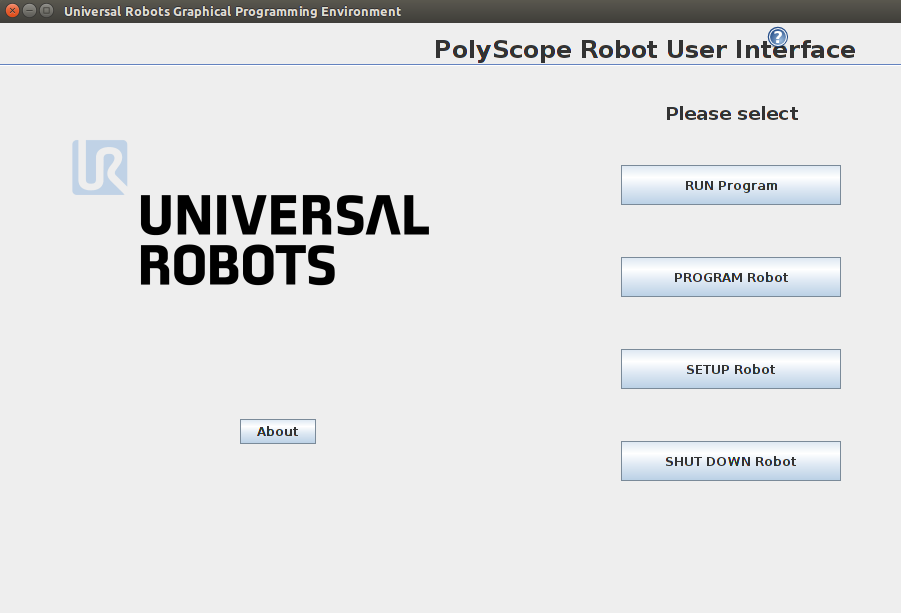
\includegraphics[trim=0cm 0cm 0cm 0cm, scale=0.4]{screenshots_tuto_ursim/interface_init.png}
  \end{tabular}
 \end{center}
\caption{Interface initiale d'URsim}
 \label{fig:ui_start}
\end{figure}

\begin{itemize}
\item Le bouton \textit{RUN Program} permet de faire fonctionner des routines contenant différentes fonctions. Ces routines sont communément appelées \textit{URscript}. Ces scripts peuvent variés en complexité allant d'une simple séquence de positions à atteindre jusqu'à un programme complexe gérant de multiples sockets de communications UDP et répondant à des appels de fonctions listées dans la librairie d'URsim.
\item Le bouton \textit{PROGRAM Robot} permet la rédaction ou la modification d'URscripts
\item Le bouton \textit{SETUP robot} permet la modification de paramètres tels que l'adresse IP d'un robot réel qu'un utilisateur voudrait contrôler via l'instance d'URsim installée sur la machine virtuelle.
\end{itemize}

Quand un utilisateur charge un URscript, il appui alors sur \textit{PROGRAM ROBOT}, puis sur \textit{Load Program} (ou sur \textit{Empty program} si il n'y a pas de programmes déjà disponibles). Une fois cette opération complétée la fenêtre présente à la Figure \ref{fig:ui_programmation}. Ceci constitue l'interface de programmation d'URscripts. Un manuel de programmation URscript est inclue dans l'appendice A, cependant, pour le fonctionnement de l'environnement de développement tel que présenté, aucune programmation URscript ne sera nécessaire.

\begin{figure}
 \begin{center}
  \begin{tabular}{c}
    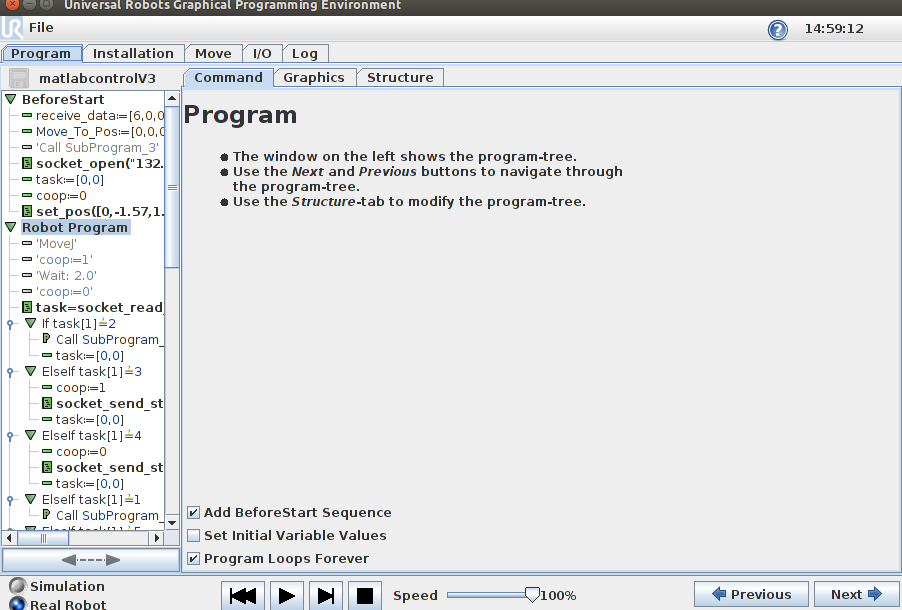
\includegraphics[trim=0cm 0cm 0cm 0cm, scale=0.35]{screenshots_tuto_ursim/interface_prog.png}
  \end{tabular}
 \end{center}
\caption{Interface de programmation d'URsim}
 \label{fig:ui_programmation}
\end{figure}



\subsection{Lien URsim-Matlab}
Comme mentionné précédemment, les URscripts peuvent gérer des sockets de communication UDP et utiliser des fonctions tirées de la librairie d'URsim. 
En premier lieu, les manipulations requises dans le logiciel URsim lancé dans la machiner virtuelle seront décrites.
Ensuite, les étapes à suivres dans l'environnement de développement Matlab sous windows seront expliquées.

\subsubsection{URsim}

C'est de cette manière qu'un URscript a été rédigé de manière à répondre à certaines commandes envoyées sous format texte par Matlab.
Les fichiers URscripts en question sont disponibles dans le dossier \textit{programs} du dépot github \href{https://github.com/wonwon0/sujet_special_gmc.git}{suivant}.
Pour rendre ces URscripts disponibles pour URsim, il faut seulement remplacer le dossier \textit{programs} présent dans le répertoire d'instalation d'URsim par celui téléchargé depuis le répertoire github mentionné plus haut. La figure \ref{fig:programs} représente grosso modo l'endroit dans lequel il faut remplacer le dossier \textit{programs}.
\begin{figure}
 \begin{center}
  \begin{tabular}{c}
    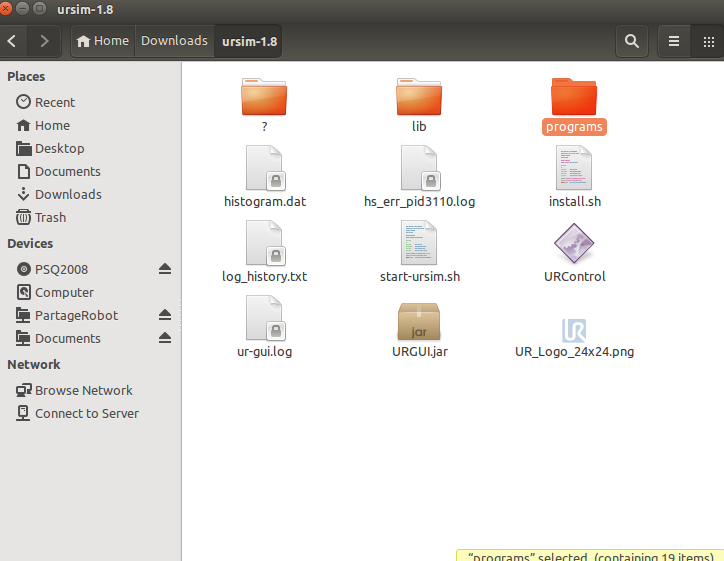
\includegraphics[trim=0cm 0cm 0cm 0cm, scale=0.4]{screenshots_tuto_ursim/programs.png}
  \end{tabular}
 \end{center}
\caption{Emplacement du dossier \textit{programs}}
 \label{fig:programs}
\end{figure}

Suivant le dépot du dossier \textit{programs} dans le répertoire d'URsim, il est possible d'ouvrir le programme portant le nom d'\textit{matlabcontrolV3.urp} après avoir sélectionné \textit{Load Program} tel que vu dans la Figure \ref{fig:ui_start}.

Ensuite, il faut executer les étapes suivante:
\begin{itemize}
\item Modifier l'adresse IP dans la fonction \textit{socket\_open} du URscript pour qu'elle concorde avec l'adresse IP du controleur réseau de VMware. Cette infromation est disponible en ouvrant un invité de commande dans la session Windows et de tapper ipconfig. La Figure \ref{fig:windows_ip} représente la sortie de l'invité de commande qu'il faut remarquer lors de l'Entrée de la commande ipconfig.
\item Sélectionner l'option \textit{Simulation} dans le bas de la fenêtre d'URsim.
\item Appuyer sur le bouton \textit{Play} présent de le bas, au centre, de la fenêtre d'URsim.
\end{itemize}
\begin{figure}
 \begin{center}
  \begin{tabular}{c}
    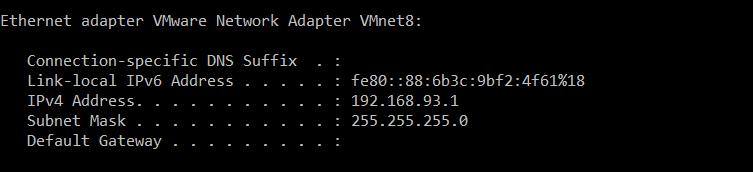
\includegraphics[trim=0cm 0cm 0cm 0cm, scale=0.5]{screenshots_tuto_ursim/windows_ip.png}
  \end{tabular}
 \end{center}
\caption{Exemple de l'adresse ip du contrôleur de VMware qu'il faut prendre en note (IPv4 address)}
 \label{fig:windows_ip}
\end{figure}
Ces étapes lancent l'URscript sur un robot virtuel et permet l'écoute et la réponse à des commandes envoyées par Matlab.


\subsubsection{Matlab}

Une fois l'environnement virtuel d'URsim mis en place, l'environement matlab requis pour communiquer avec URsim doit être implémenté.
Un environnement de travail matlab situé dans le répertoire github mentionné plus dans la dernière section contient plusieurs fichiers nécessaires à la communiquation avec URsim, VRep et ROS, un environnemnt dont le présent document traite dans une autre section.




\subsection{Logiciel de visualistion VRep}

Bien que le logiciel URsim permet de représenter le robot dans un environnement 3D de base, il ne permet pas la représentation d'objets composant l'environnement de travail du robot.
Pour se faire, le logiciel VRep est utilisé.
Ce dernier permet d'afficher une multitude d'objets localisés dans une librairie déjà prédéfinie.
Cette section couvre brièvement les étapes requise pour l'instalation et l'utilisatiuon de VRep avec matlab.

\subsubsection{Instalation de VRep}

L'instalation de VRep peut se faire rapidement en téléchargeant la version d'éducation sur le site web officiel \href{http://www.coppeliarobotics.com/downloads.html}{suivant}.

\subsection{Interface matlab-VRep}

Suite à l'instalation de VRep, 

\newpage
























 